\documentclass[a4paper, 12pt]{article}
%\usepackage[OT2, T1]{fontenc}
\usepackage[utf8]{inputenc}
\usepackage{amsmath}
\usepackage{amssymb}
\usepackage{minted}
\usepackage[utf8]{inputenc}
\usepackage[T2A]{fontenc}
\usepackage[unicode, pdftex]{hyperref}
\usepackage[russian, english]{babel}
\usepackage{comment}
\usepackage{subfiles}
\usepackage{pxfonts}
\usepackage{environ}
\usepackage{changepage}
\usepackage{physics}
\usepackage[fleqn,tbtags]{mathtools}
\usepackage{setspace}
\usepackage{ragged2e}
\usepackage{blindtext}
\usepackage{microtype}
\singlespacing
\usepackage[left=1cm,right=1cm,top=1cm,bottom=1cm,bindingoffset=0cm]{geometry}


\begin{document}
\begin{center}
\noindent
{\fontsize{14pt}{18pt}\selectfont 
	\pmb{Исследование многофазной RQ-системы массового обслуживания с общей орбитой.} \\
	Исаев Кимал Илхам оглы} \\ 
\pmb{Томский Государственный Университет, г. Томск, Российская Федерация} \\
\pmb{Бакалавр - 4 курс}
\end{center}

\noindent
\hspace{1cm}
Рассматривается система массового обслуживание с простейшим входящим потоком, интенсивность которого равняется \(\lambda\), с общей орбитой, на которой интенсивность каждой заявки равна \(\sigma\), и N приборов, каждый из которых имеет гиперэкспоненциальное М-фазное распределения с вероятностями перехода на k-ую фазу \(q_k\), где \(\sum_{k=1}^M q_k = 1\), а время пребывания заявки на k-ой фазе распределено по экспоненциальному закону с параметром \(\mu_k\), при окнчании обслуживания с вероятность \(r_0\) заявка выходит из системы, с вероятностью \(r_1\) поступает на мгновенное повторное обслуживание, где снова определяется фаза для обслуживания, с вероятностью \(r_2\) поступает на общую орбиту для отложенного повторного обслуживания, причём \(r_0 + r_1 + r_2 = 1\).
\\
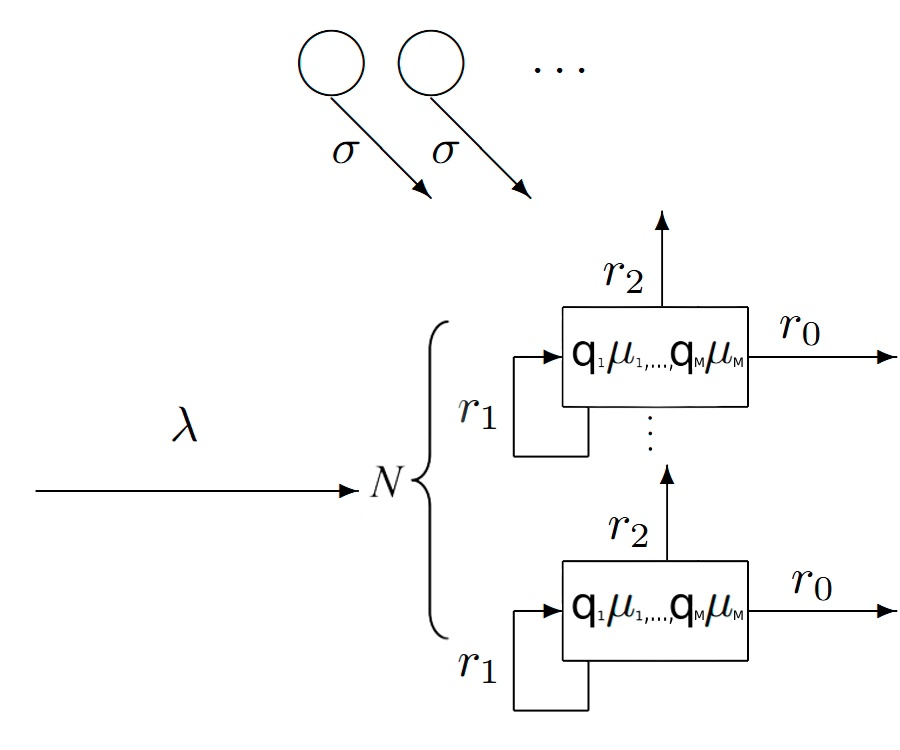
\includegraphics[scale=0.5]{NExecutionMPhase}

\noindent
\hspace{1cm}
В результате исследования получен алгоритм вычисления аппроксимации распределения количества заявок на орбите в стационарном режиме для любой марковской RQ-системы массового обслуживания с общей орбитой при заданых постоянных интенсивностях изменения состояния системы, кроме интенсивности убывания заявок с орбиты, что должна быть линейно зависима от количества заявок на орбите, с нулевым свободным коэффицентом, при ординарном поступлении заявок на орбиту и ординарном убывании заявок с орбиты. После чего доказывается применимость данного алгоритма для системы массового обслуживания описанной выше и сравниваются полученные результаты с результатами имитационного моделирования.
\end{document}
